% !TEX encoding = UTF-8
% !TEX TS-program = pdflatex
% !TEX root = ../tesi.tex

%**************************************************************
\chapter{Performance}
\label{cap:performance}
%**************************************************************
\section{Confronto dei vari metodi}
In questa sezione confronteremo il tempo di esecuzione dei vari metodi risolutivi per 5 configurazioni iniziali del problema, di difficoltà crescente dal livello 0 al livello 4.\\
Per i primi 4 problemi abbiamo anche un dato del tempo impiegato da una persona nel risolvere il problema. Abbiamo infatti sottoposto i vari livelli a 8 persone diverse, di età compresa tra 16 e 55 anni, cronometrandoli durante lo svolgimento del gioco.\\
Per ogni livello è presente una tabella che contiene le misure di performance, in termini di tempo medio di esecuzione, rilevate per ogni tipo di solver; inoltre tra parentesi è presente il numero medio di stati attraversati da ogni solver per arrivare allo stato obiettivo. \\
Per ogni tabella, si paragonano tra loro i risultati ottenuti da ogni solver con o senza le migliorie specificate in \ref{migliorie}

\subsection{Livello 0}
La configurazione iniziale del livello 0 è mostrata in figura \ref{lev0}. Le forme mancanti da inserire sono mostrate nelle figure \ref{z}, \ref{c}, \ref{y}.
\begin{figure}[h]
	\centering
	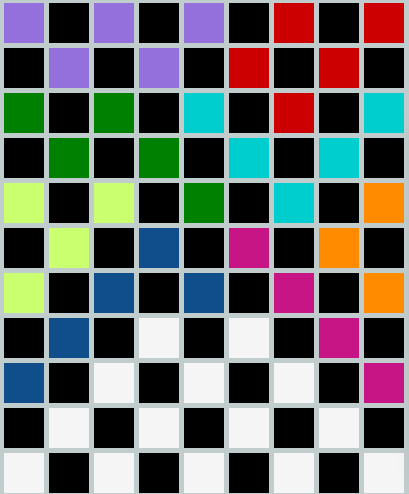
\includegraphics[scale=0.3]{immagini/lv0}
	\caption{Livello 0}
	\label{lev0}
\end{figure}
\\
\noindent

\begin{table}[h] 
	\begin{tabular}{|l||*{4}{c|}}\hline 
		\backslashbox{Miglioria}{Solver} 
		&\makebox{DFS}&\makebox{Backtracking}&\makebox{Recursive Backtracking}	&\makebox{MinConflicts}\\ \hline 
		Sì&0.0192 (4.0)&0.0857 (11.0)&0.0708 (11.0)&0.0264 (1.0) \\ \hline 
		No&0.0786 (30.0)&0.0319 (11.0)&0.0327 (11.0)&0.0208 (1.0)  \\ \hline 
	\end{tabular}
	\caption{Tempi di esecuzione in secondi del livello 0} 
\end{table}

\subsubsection{Osservazioni}
Possiamo notare come a partire da questa configurazione, dove mancano solamente 3 forme da inserire e quindi lo spazio di ricerca è molto limitato, l'algoritmo migliore risulta essere DFS con la miglioria del Connected Component Check, in quanto questo controllo elimina dai domini tutti i valori non consistenti ottenendo così una soluzione mediamente in soli 4 assegnamenti (dai 30 ottenuti senza questo controllo).\\
Per quanto rigurda gli altri solver, essendo il problema relativamente semplice, il Connected Component Check porta un peggioramento delle prestazioni in quanto introduce complessità aggiuntiva ad ogni assegnamento, senza diminuirne il numero significativamente.

\subsection{Livello 1}
La configurazione iniziale del livello 1 è mostrata in figura \ref{lev1}. Le forme mancanti da inserire sono mostrate nelle figure \ref{z}, \ref{c}, \ref{y}, \ref{w}.
\begin{figure}[h]
	\centering
	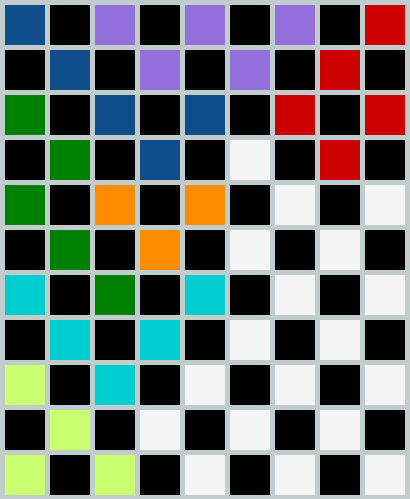
\includegraphics[scale=0.3]{immagini/lv1}
	\caption{Livello 1}
	\label{lev1}
\end{figure}
\\
\noindent
\begin{table}[h]
	\begin{tabular}{|l||*{4}{c|}}\hline 
		\backslashbox{Miglioria}{Solver} 
		&\makebox{DFS}&\makebox{Backtracking}&\makebox{Recursive Backtracking}	&\makebox{MinConflicts}\\ \hline 
		Sì&0.0483 (9.66666)&0.1135 (12.0)&0.1104 (12.0)&0.0668 (1.0) \\ \hline 
		No&0.2974 (147.5)&0.0480 (12.0)&0.0506 (13.0)&0.0910 (1.0)  \\ \hline 
	\end{tabular} 
	\caption{Tempi di esecuzione in secondi del livello 0} 
\end{table}

\subsubsection{Osservazioni}
I risultati ottenuti nel livello 1 rispecchiano quelli del livello precedente, in quanto anche in questo caso lo spazio degli stati è molto limitato (solo 4 forme da inserire). Da notare come il Connected Component Check diminuisca in media da 147 a 9 gli assegnamenti nel caso dell'algoritmo DFS, con un notevole risparmio di tempo.

\subsection{Livello 2}
La configurazione iniziale del livello 2 è mostrata in figura \ref{lev2}. Le forme mancanti da inserire sono mostrate nelle figure \ref{p}, \ref{smallv}, \ref{bigz}, \ref{i}, \ref{w}, \ref{v}.
\begin{figure}[h]
	\centering
	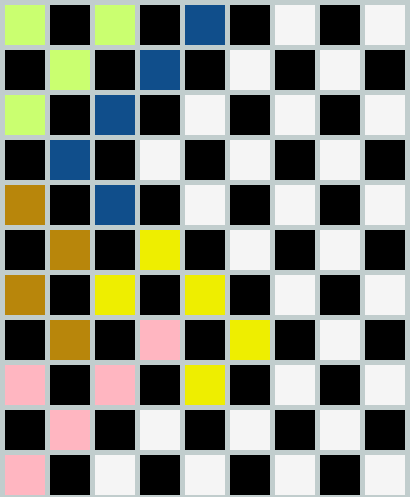
\includegraphics[scale=0.3]{immagini/lv2}
	\caption{Livello 2}
	\label{lev2}
\end{figure}
\\
\noindent
\begin{table}[h]
	\begin{tabular}{|l||*{4}{c|}}\hline 
		\backslashbox{Miglioria}{Solver} 
		&\makebox{DFS}&\makebox{Backtracking}&\makebox{Recursive Backtracking}	&\makebox{MinConflicts}\\ \hline 
		Sì&0.3546 (78.3333)&0.1969 (22.0)&0.1874 (17.0)&0.3349 (1.0) \\ \hline 
		No&1.8782 (1472.5)&0.1241 (32.0)&0.0984 (19.0)&0.2641 (1.0)  \\ \hline 
	\end{tabular} 
	\caption{Tempi di esecuzione in secondi del livello 0} 
\end{table}

\subsubsection{Osservazioni}
In questo esercizio il numero di forme da inserire è 6, generando così uno spazio degli stati notevolmente maggiore.
La prima cosa da notare è che l'algoritmo DFS inizia a diventare poco efficiente, sia dal punto di vista del numero di azioni da eseguire, sia come tempi di esecuzioni

\subsection{Livello 3}
La configurazione iniziale del livello 3 è mostrata in figura \ref{lev3}. Le forme mancanti da inserire sono mostrate nelle figure \ref{z}, \ref{smallv}, \ref{bigz}, \ref{c}, \ref{y}, \ref{t}, \ref{w}, \ref{v}.
\begin{figure}[h]
	\centering
	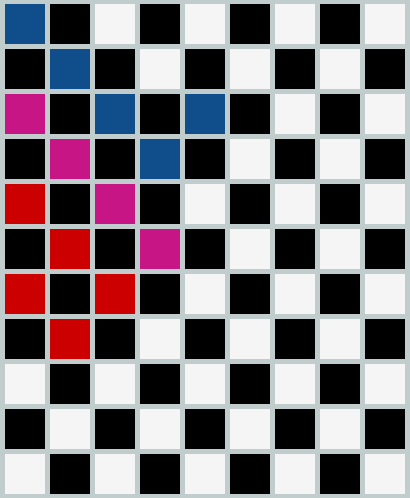
\includegraphics[scale=0.3]{immagini/lv3}
	\caption{Livello 3}
	\label{lev3}
\end{figure}
\\
\noindent

\begin{table}[h] 
	\begin{tabular}{|l||*{4}{c|}}\hline 
		\backslashbox{Miglioria}{Solver} 
		&\makebox{DFS}&\makebox{Backtracking}&\makebox{Recursive Backtracking}	&\makebox{MinConflicts}\\ \hline 
		Sì&36.227 (12343.8)&1.5018 (198.0)&0.5316 (55.0)&40.468 (15.1666) \\ \hline 
		No&1786,2 (312.000)&1.3156 (1179.0)&0.8229 (572.0)& ()  \\ \hline 
	\end{tabular} 
	\caption{Tempi di esecuzione in secondi del livello 0} 
\end{table}


\subsection{Livello 4}
La configurazione iniziale del livello 4 è mostrata in figura \ref{lev4}. Tutte le forme devono essere inserite nella griglia.
\begin{figure}[h]
	\centering
	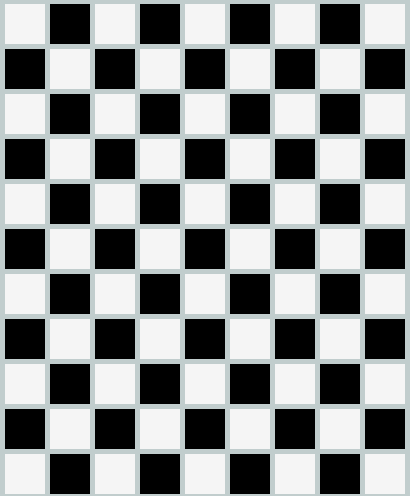
\includegraphics[scale=0.3]{immagini/lv4}
	\caption{Livello 4}
	\label{lev4}
\end{figure}
\\
\noindent

\begin{table}[h] 
	\begin{tabular}{|l||*{4}{c|}}\hline 
		\backslashbox{Miglioria}{Solver} 
		&\makebox{DFS}&\makebox{Backtracking}&\makebox{Recursive Backtracking}	&\makebox{MinConflicts}\\ \hline 
		Sì& ()&1.4544 (184.0)&16.338 (2640.0)&24.502 (5.42857) \\ \hline 
		No& ()&5.1879 (4002.0)&26.403 (23971.0)& ()  \\ \hline 
	\end{tabular} 
	\caption{Tempi di esecuzione in secondi del livello 0} 
\end{table}



